
As discussed in Section~\ref{sec:introduction}, the term \enquote{trending} denotes the alignment of a detected true development with the development indicated by another measurement, a nowcast, or a forecast.
In this section, we want to specify trending and define different methods of measuring and visualizing trending.
Development always has respect to a time horizon, that is, the amount of time passed during development. 
In general, trending can be assessed for different horizons $l$ separately, and the considered horizons' relevance must be determined based on the question at hand.
Throughout the section, we call a measurement, nowcast, or forecast a \textit{prediction} or \textit{signal} whenever the application area is insignificant.
Before introducing measures to evaluate trending, we remark on calculating the predicted change and notation in Section~\ref{subsec:notation}.
Section~\ref{subsec:trending-basics} introduces trending basics and visualizes trending in a synthetic example.
In Section~\ref{subsec:trending-measures}, various methods from other disciplines and tasks are applied and examined.
The approaches are extended to account for noise and non-systematic effects in Section~\ref{subsec:trending-noise}.
Section~\ref{subsec:trending-cond-prob} introduces a new graphical method for local trending assessment and briefly introduces bootstrap methods for computing confidence intervals for the measures in the previous sections.
Trending assessment for probabilistic nowcasts and forecasts is treated in Section~\ref{subsec:probabilistic}.

\subsection{Computing changes and notation}\label{subsec:notation}

As noted above, trending refers to observed and predicted changes over a time horizon $l$.
The \textit{observed} change is straightforward to compute for all types of signals.
Let $\mathbf{y} = (y_t)_{t=0}^T$ denote the true values for nowcasting or forecasting, or gold standard measurements up to time $T$.
The sequence of observed changes is then given by the differences of values in $\mathbf{y}$ with horizon $l$, that is
\begin{equation}\label{eq:diffy}
    \diffylt = (y_{t} - y_{t-l}) \quad \text{for}\ t = l, \dots, T.
\end{equation}

\begin{table}
    \centering
    \scriptsize
    \begin{tabularx}{0.75\textwidth}{l X}
        \toprule
        Application & Predicted change computation \\
        \midrule
        Measurement & $(x_{t} - x_{t-l})_{t=l}^T $\\
        Nowcasting & $
\diffxl =
\begin{cases}
(x_{t|t} - x_{t-l|t})^T_{t=l}, & \text{if } y_{t-l} \text{ is not known at time } t, \\
(x_{t|t} - y_{t-l})^T_{t=1}, & \text{otherwise}.
\end{cases} 
$ \\
        Forecasting & $ \diffxl = (x_{t|t-l} - y_{t-l})^T_{t=l}$\\
        \bottomrule
    \end{tabularx}
    \caption{Computation of the predicted change in the different applications. For nowcasting and forecasting, signals $x_{t | \tau}$ refer to values issued at $\tau$ with a target time $t$. For measurement, $x_t$ denotes the test device measurement at time $t$.}
    \label{tab:notation}
\end{table}


The definition of the predicted change depends on the context.
Table~\ref{tab:notation} summarizes the notation for the different signal types and the computation of the predicted change.
For nowcasting, let $x_{t | \tau}$ denote the nowcast for time $t$ computed with the knowledge of time $\tau$. 
We call $t$ the \textit{forecast time} and $\tau$ the \textit{issue time}.
We compute the predicted change by
\begin{equation}
  \diffxl =
\begin{cases}
(x_{t|t} - x_{t-l|t})^T_{t=l} & \text{if } y_{t-l} \text{ is not known at time } t, \\
(x_{t|t} - y_{t-l})^T_{t=1} & \text{otherwise}.
\end{cases} \label{eq:diffxl_nowcasting}
\end{equation}
When computing the predicted change of a nowcast for a time $t$, we use the best knowledge available at that time $t$, and the true value might not be known yet. 
Thus, the predicted can be computed with the knowledge of time $t$, and the trending assessment can be used in practice at time $t$.

The notation is similar for forecasting: Let $x_{t | \tau}$ denote the forecast for forecast time $t$ and issue time $\tau$. 
The predicted change is computed by 
\begin{equation} \diffxl = (x_{t|t-l} - y_{t-l})^T_{t=l} \label{eq:diffxl_forecasting}
\end{equation}
The indices are chosen to be consistent with $\diffyl$. 
If the true value $y_{t-l}$ is not known at time $t-l$, a similar modification can be made as in Equation~\eqref{eq:diffxl_nowcasting}.


The distinction between forecast and issue time is unnecessary in measurement analysis, as the measurement is typically available with a very short time lag. 
Thus, $x_t$ denotes the test method measurement for time $t$. 
The computation
\begin{equation}
  (x_{t} - x_{t-l})_{t=l}^T \label{eq:diffxl_measure}
\end{equation}
yields the change by the test method. 
It is computed purely by the test method without the gold standard $y_t$ to analyze whether the gold standard and test method changes are consistent.

\subsection{Basics of trending and four-quadrant plots}\label{subsec:trending-basics}

The trending assessment is the same for all three application areas, given the notation for the respective application of Section~\ref{subsec:notation}.
In the following, we omit the difference horizon $l$ for ease of notation; $\diffx$ and $\diffy$ refer to $\diffxl$ and $\diffyl$ for a common horizon $l$ as defined in Table~\ref{tab:notation}.
As noted above, a signal's trending is perfect if all the change directions are predicted correctly; that is, the sign of all elements of $\diffx$ and $\diffy$ coincide.
Consequently, when evaluating the trending, we examine the statistical consistency of $\sign(\diffx)$ and $\sign(\diffy)$.
A simple yet insightful method is the four-quadrant plot~\parencite[see, e.g., ][]{Saugel2015,perrino1998intraoperative}. 
In a four-quadrant plot, the occured changes are plotted with the predicted changes, that is, $(\diffy_t, \diffx_t)$ for $t = 1, \dots, T$.
Thus, the x-axis of a four-quadrant plot shows the true value differences, whereas the y-axis displays the prediction data differences.
Points in the green upper right and lower left quadrants reflect a correct trending for the respective time step, whereas points in the remaining red quadrants show incorrect predicted changes.

Figure~\ref{fig:trending_basic_4q} displays a basic four-quadrant plot.
Points 2, 3, 5, and 6 show trending, whereas points 1, 4, and 7 count for anti-trending behavior.
Figure~\ref{fig:trending_basic_4q_sample} shows a four-quadrant graph for a more extensive simulated data set with $T=1461$, for example, four years of daily data.
Data generation is described in Appendix~\ref{subsec:app-trending-data-generation} and will continue into this section.
The four-quadrant plot resembles a butterfly-like shape, with more data in the upper right and lower left quadrants than in the remaining quadrants.

The four-quadrant plot is intuitive to interpret, and the magnitude and direction of change are shown simultaneously.
It can be extended by including information on the date in the point color.
In Figure~\ref{fig:trending_basic_4q_sample_color}, the point colors turn from blue to green for higher time indices $t$.
The horizon is always one time step.
However, four-quadrant plots become crowded for larger datasets, and sequential information on the differences is complex to assess thoroughly.
There are other visualization techniques, such as polar plots or the Bland-Altmann analysis.
However, they lack the four-quadrant plot's clarity and intuition without adding more information on trending~\parencite{Saugel2015}.

\begin{figure}
\centering
\begin{subfigure}[t]{.24\textwidth}
\includegraphics{plots/illustrative_examples/4Q_without_excl}
\caption{Basic four-quadrant plot.} \label{fig:trending_basic_4q}
\end{subfigure}\hspace{0.01\textwidth}%
\begin{subfigure}[t]{.24\textwidth}
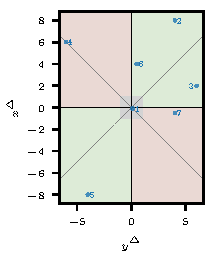
\includegraphics{plots/illustrative_examples/4q_excl_box}
\caption{Four-quadrant plot with rectangular exclusion area.}\label{fig:trending_basic_4q_excl_box}
\end{subfigure}\hspace{0.01\textwidth}%
\begin{subfigure}[t]{.24\textwidth}
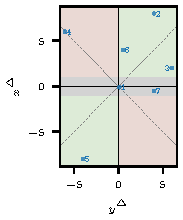
\includegraphics{plots/illustrative_examples/4q_excl_axis}
\caption{Four-quadrant plot with horizontal exclusion area.} \label{fig:trending_basic_4q_excl_axis}
\end{subfigure}\hspace{0.01\textwidth}%
\begin{subfigure}[t]{.24\textwidth}
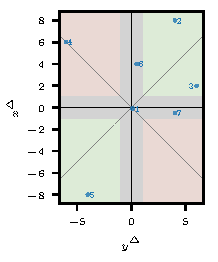
\includegraphics{plots/illustrative_examples/4q_excl_cross}
\caption{Four-quadrant plot with cross-shaped exclusion area.}\label{fig:trending_basic_4q_excl_cross}
\end{subfigure}%
\caption{Illustrations of the four-quadrant plot with sample points and with and without exclusion areas. }
\label{fig:trending_4q}
\end{figure}

\subsection{Trending ratio and other measures}\label{subsec:trending-measures}

Analyzing the number of points in the green versus red quadrants is a standard approach in the trending assessment of measurement data \parencite{Critchley2010,Saugel2015}. 
With that, we mainly estimate the probability of trending $P(\diffxrv \diffyrv > 0)$, where $\diffyrv$ and $\diffxrv$ denote random variables for future incremental changes.
Note that $z_1 z_2 > 0$ if and only if $\sign(z_1) = \sign(z_2)$ ($z_1, z_2 \in \R \setminus \{ 0 \}$).
The standard estimator for $P(\diffxrv \diffyrv > 0)$ is
\begin{equation}
    \acc (\diffx, \diffy) \coloneqq \frac{\sum_{t \in \mathcal{T}} \ind{\diffxt \diffyt > 0}}{\card{T}}.\label{eq:acc}
\end{equation}
The numerator counts the number of same-sign-changes, while the denominator is the number of all points.
Thus, $\acc$ is the ratio of concordant changes over all changes.
We refer to this estimator as the trending ratio of the prediction and set $\mathcal{T} = \{l, \dots, T\}$. 
Visually, the measure computes the fraction of points in the upper right or lower left quadrant.
Such a $2 \times 2$ table of counts is called a contingency table.
It is often used in other scientific areas for evaluation, for example, in dichotomous forecasting or as a confusion matrix in classification analysis~\parencites(see, e.g., the introductions in)()[Ch. 4]{James2021}[Ch. 3]{Jolliffe2012}.
There, a wide range of other methods are usually used to analyze further characteristics of contingency tables.
Two simple measures that focus on either a positive or negative predicted change are the positive and negative trending ratios $\accp$ and $\accm$, respectively.
They are defined as
\begin{align}
    \accp (\diffx, \diffy) &\coloneqq \frac{\sum_{t \in \mathcal{T}} \ind{\diffxt \diffyt > 0} \ind{\diffxt > 0}}{\sum_{t \in \mathcal{T}} \ind{\diffxt > 0}} \label{eq:accp}\\
    \accm (\diffx, \diffy) &\coloneqq \frac{\sum_{t \in \mathcal{T}} \ind{\diffxt \diffyt > 0} \ind{\diffxt < 0}}{\sum_{t \in \mathcal{T}} \ind{\diffxt < 0}}\label{eq:accm}
\end{align}
In the classification context, these measures are known as positive or negative predictive value and hit rate or detection failure ratio in forecasting.
They give the probability of a correct prediction of the direction of change, given that the signal direction is positive or negative, respectively, that is, $P(\diffxrv \diffyrv > 0 | \diffxrv > 0)$ and $P(\diffxrv \diffyrv > 0 | \diffxrv < 0)$, respectively.

Rolling estimates of the above measures detect changes in performance over time and can give a sharper estimate of the current trending ability.
For the trending ratio, a rolling estimate with a backward-looking window of length $w$ at time $t$ is given by
\begin{equation*}
    \acc_{t; w} (\diffx, \diffy) \coloneqq \frac{\sum_{t^\star = t-w + 1}^{t} \ind{\diffxt[t^\star] \diffyt[t^\star] > 0}}{w}.\label{eq:acc_rolling}
\end{equation*}
Backward-looking windows provide an estimate at a time $t$ considering the $w$ time steps before time $t$.
The window length $w$ controls the smoothing of the estimate, a larger $w$ gives smoother results, while a small $w$ focus on local variations.
Plotting the rolling estimates for $t = w-1, \dots, T$ yields an estimate of the trending ability over time.
Figure~\ref{fig:trending_ratio_time_series} depicts a rolling window estimate of the trending ratio for the simulated data of Figures~\ref{fig:trending_basic_4q_sample} and~\ref{fig:trending_basic_4q_sample_color}.
Thus, the yearly course of the prediction trending ratio can be detected.
The trending ability of the signal has a strong sinus-shaped seasonality with a trending ability peak after a quarter of a year and a low point after three quarters.
This seasonal behavior cannot be distinguished in the two four-quadrant plots or the trending ratio.


\begin{figure}
    \centering
    \begin{subfigure}[t]{.24\textwidth}
\includegraphics{plots/illustrative_examples/4Q_sample_without_time}
\caption{Four-quadrant plot with simulated data.}\label{fig:trending_basic_4q_sample}
\end{subfigure}\hspace{0.01\textwidth}
\begin{subfigure}[t]{.24\textwidth}
\includegraphics{plots/illustrative_examples/4Q_sample_with_time}
\caption{The same data is colored according to the time index $t$, the greener, the later.}\label{fig:trending_basic_4q_sample_color}
\end{subfigure}\hspace{0.01\textwidth}
\begin{subfigure}[t]{.48\textwidth}
    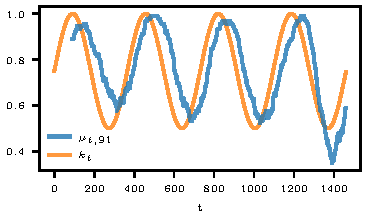
\includegraphics{plots/illustrative_examples/trending_ratio_time_series.pdf}
    \caption{Rolling estimate of the trending ratio over time with window length 91. }\label{fig:trending_ratio_time_series}
    \end{subfigure}%
    \caption{Visualizations for data with a time-varying trending ratio. We defer information on the data generation process in \ref{fig:trending_basic_4q_sample} and \ref{fig:trending_basic_4q_sample_color} to the appendix (see \ref{subsec:app-trending-data-generation}). The trending ratio for the entire data set is $\mu = 0.7577$. The strong seasonality of the trending ratio becomes visible in Figure~\ref{fig:trending_ratio_time_series}. The green curve $k_t$ shows the probability that $\diffxt$ has the same sign as $\diffyt$ for each time step. The rolling estimates are delayed as the windows look backward.}
\end{figure} 

In applications, signal data are often not available for all time steps, for example, due to technical problems or delays in data transfer (see the examples in Sections~\ref{sec:application-covid} and~\ref{sec:application-eda}).
We refer to time steps for which either signal or true values or both are unavailable as missing values.
Data pairs with missing values can be excluded from the set $\mathcal{T}$ to calculate the measures. 
However, systematical missing values could lead to a biased estimate of the trending ratio, for example, if signal data is omitted in times of high change and thus uncertainty.
In this case, measures should be interpreted cautiously, and inspection of missing data should accompany applications with missing data, for example, through a visual assessment.
In the applications in Sections~\ref{sec:application-covid} and~\ref{sec:application-eda}, only a few missing values occur, and we provide information on the missing data by inspecting the missing data as lists.

\subsection{Accounting for noise and non-informative small changes and bootstrap confidence intervals}\label{subsec:trending-noise}

The above measures can be extended to account for information on the points location within the quadrant.
For example, points close to the zero point may have less explanatory power or are less reliable than points far away from zero on one of the diagonals.
Suppose noise or non-systematic effects are present in the true values or predictions. 
In that case, a point's assignment to a quadrant can be driven by noise instead of a systematic trending ability of the signal.
This happens more frequently for points with at least one small coordinate.

Using an exclusion area around the zero point as further defined below is a straightforward and highly interpretable extension of the measures of Section~\ref{subsec:trending-measures}.
Points within that area are neither plotted in the four-quadrant plot nor included in the calculation of the measures.
In general, it is likely that the prediction models have a noise component and should thus be part of the exclusion area.
We denote the measures of Equations~\eqref{eq:acc},~\eqref{eq:accp} and~\eqref{eq:accm} accounting for an exclusion area $E$ by
\begin{align}
    \acceps (\diffx, \diffy, E) &\coloneqq \frac{\sum_{t \in \mathcal{T}} \ind{\diffx \diffy > 0} \ind{(\diffyt, \diffxt) \notin E}}{\sum_{t \in \mathcal{T}} \ind{(\diffyt, \diffxt) \notin E}}\label{eq:acceps}\\
    \accpeps (\diffx, \diffy, E) &\coloneqq \frac{\sum_{t \in \mathcal{T}} \ind{\diffxt \diffyt > 0} \ind{\diffxt > 0, , (\diffyt, \diffxt) \notin E}}{\sum_{t \in \mathcal{T}} \ind{\diffxt > 0, (\diffyt, \diffxt) \notin E}} \label{eq:accpeps}\\
    \accmeps (\diffx, \diffy, E) &\coloneqq \frac{\sum_{t \in \mathcal{T}} \ind{\diffxt \diffyt > 0} \ind{\diffxt < 0, (\diffyt, \diffxt) \notin E}}{\sum_{t \in \mathcal{T}} \ind{\diffxt < 0, (\diffyt, \diffxt) \notin E}}\label{eq:accmeps}
\end{align}
The measures are then estimators for the probability of trending, given that the change is not in the exclusion area $E$, that is, for $\acceps$, $P(\diffxrv \diffyrv > 0 | \diffxrv \diffyrv \notin E)$.
The estimators accept various shapes of the exclusion area.
Figure~\ref{fig:trending_4q} visualizes examples of the exclusion area.
A rectangular exclusion area, $E = \{(x, y) \in \R^2: (-\varepsilon_x \leq x \leq \varepsilon_x) \land (-\varepsilon_y \leq y \leq \varepsilon_y) \}$ 
 ($\varepsilon_x, \varepsilon_y > 0$), leaves out points that are small in both components and, therefore, likely to be driven by noise.
Points where at least the true value or signal is unlikely to be zero are not excluded.
In the example graph in Figure~\ref{fig:trending_basic_4q_excl_box}, only point 1 is excluded.
An exclusion area along one axis, for example, $E = \{(x, y) \in \R^2: (-\varepsilon_x \leq 0 \leq \varepsilon_x)\}$ for $\varepsilon_x > 0$, removes points in which one of the components could change sign by a small amount of noise.
This particularly suits signals where small amounts of noise are inevitable.
A cross-shaped exclusion area, $E = \{(x, y) \in \R^2: (-\varepsilon_x \leq x \leq \varepsilon_x) \lor (-\varepsilon_y \leq y \leq \varepsilon_y) \}$ for $\varepsilon_x, \varepsilon_y > 0$, along both axes accounts for the sign reversal in both components.
For these two methods, points 1 and 7 in Figure~\ref{fig:trending_basic_4q_excl_axis} or 1, 6, and 7 are excluded in Figure~\ref{fig:trending_basic_4q_excl_cross}, respectively.

In most applications, the shape and size of the exclusion area can be chosen based on domain knowledge or expert opinions.
The size estimation can also be based on a proportion of the total variance or the total range of the data, for example, the points with at least one coordinate in the smallest 10\% of absolute values are excluded.
A third approach is to visualize the trending ratio for different sizes of $E$ and thus inspect the effects of the exclusion area size on the estimates.
For examples on those plots, see Section~\ref{sec:application-covid}.

Confidence intervals can account for the estimation uncertainty of the measures above.
Bootstrap confidence intervals are a nonparametric technique based on resampling~\parencite[for introductions see][]{Hesterberg2011,Bittmann2021}.
New samples are drawn with replacement from the dataset and are not based on parametric assumptions as classical confidence intervals are.
The confidence interval is then computed based on those bootstrap samples.
We use the \ac{bca} approach for bootstrapping in the following, as it hold the confidence level for small and large samples and has a moderate computation time (see the simulation study in Appendix~\ref{subsec:appendix-trending-bootstrap}).


\subsection{The conditional trending plot}\label{subsec:trending-cond-prob}

The estimators described above give information on the probabilities $P(\diffxrv \diffyrv > 0 | \diffxrv \diffyrv \notin E)$, $P(\diffxrv \diffyrv > 0 | \diffxrv > 0, \diffxrv \diffyrv \notin E)$ and $P(\diffxrv \diffyrv > 0 | \diffxrv < 0, \diffxrv \diffyrv \notin E)$.
A still more fine and local analysis might be gained by considering the conditional distribution $P(\diffxrv \diffyrv > 0 | \diffxrv = x)$ to assess the local trending ability of a prediction.
A multivariate \acf{kde} facilitates a continuous estimation of $P(\diffxrv \diffyrv > 0 | \diffxrv = x)$ by estimating the components $f_{\diffxrv, \diffyrv}$ and $f_{\diffxrv}$ of
\begin{align*}
P(\diffxrv \diffyrv > 0 | \diffxrv = x) = \begin{cases}
                                              \int_{-\infty}^0 \frac{f_{\diffxrv, \diffyrv}(x, y)}{f_{\diffxrv}(x)} \ \textrm{d} \: y & \text{if } x < 0, \\
                                              \int_{0}^{\infty} \frac{f_{\diffxrv, \diffyrv}(x, y)}{f_{\diffxrv}(x)} \ \textrm{d} \: y & \text{if } x > 0, \\
\end{cases}
\end{align*}
for $x \neq 0$ through a \ac{kde}.
A comprehensive introduction to multivariate \ac{kde} can be found in \textcite{Gramacki2018}, and implementations are available in many programming languages~\parencite[e.g., for  Python in][]{Seabold2010}.
The \ac{kde} yields estimates for $P(\diffxrv \diffyrv > 0 | \diffxrv = x)$ for all values of $x \in \R$.
Multivariate \ac{kde} takes a kernel and bandwidth selector as modeling parameters. 
We advise using a Gaussian kernel and the cross-validation maximum likelihood as bandwith selector (see Appendix~\ref{subsec:appendix-kde}).

Assessing $P(\diffxrv \diffyrv > 0 | \diffx = x)$ graphically eases the simultaneous evaluation of various intervals.
Furthermore, the graph facilitates the comparison of various methods in a single graph and asymmetries of $P(\diffxrv \diffyrv > 0 | \diffx = x)$ with respect to $x$ in the trending ability can be detected.
We refer to the plot as a conditional trending plot.



\subsection{Probabilistic Evaluation}\label{subsec:probabilistic}

In nowcasting and forecasting, probabilistic predictions become more popular in the recent years (see, for example, Sections~\ref{sec:application-covid} and~\ref{sec:application-eda} or the review in~\cite{Gneiting2014}).
Probabilistic predictions include a point estimate and information on the forecast uncertainty and quantiles simultaneously.
For trending analysis, probabilistic predictions also contain a probability of a positive or negative change.
In this section, we extend the trending assessment to probabilistic predictions.

Probabilistic predictions can take the form of a \ac{cdf}, \ac{pdf}, or quantiles.
The \ac{cdf} is the most general and can be used to derive the others, given they exist.
Let us first assume that the prediction is a \ac{cdf} and the horizon is large enough to know the true value when issuing the forecast or nowcast.
In the appendix, we extend the analysis for predictions given as quantiles or for unknown true values.

Let $F_{t | t-l} (x)$ denote the predicted \ac{cdf} of forecast time $t$ and issue time $t - l$, where the index is analogous to the point prediction notation of Section~\ref{subsec:notation}.
For trending assessment, we compare the probability of positive change with the occurrence of positive changes. 
A positive change occurs if any value larger than the true value $y_{t-l}$ occurs. 
As for the differences in Section~\ref{subsec:notation}, the computation differs slightly for nowcasts and forecasts.
For nowcasts, the probability is calculated by
\begin{equation*}
    p_t = 1 - F_{t | t} (y_{t-l})\quad t = l, \dots, T;
\end{equation*}
while for forecasts, it is given by
\begin{equation*}
    p_t = 1 - F_{t | t-l} (y_{t-l})\quad t = l, \dots, T.
\end{equation*}
Let $z_t$ denote the indicator that the observed change at time $t$ is positive, that is,
\begin{equation*}
    z_t = \ind{\diffyt > 0} \quad t = l, \dots, T.
\end{equation*}
The probabilistic trending evaluation is then based on the probabilities $\mathbf{p} = (p_t)_{t=l}^{T}$ and the observed changes $\mathbf{z} = (z_t)_{t=l}^{T}$.
The predictive power of $\mathbf{p}$ for $\mathbf{z}$ can be assessed using probabilistic dichotomous forecast evaluation methods.
Dichotomous forecasts predict a binary outcome, for example, a positive or negative change.
Numerical measures for forecast quality are scoring rules.

The \ac{bs} is a widely used scoring rule for dichotomous probabilistic forecasts~\parencite{Brier1950}.
It is defined as
\begin{equation*}
    BS (\mathbf{p}, \mathbf{z}) = \frac{1}{T-l} \sum_{t=l}^{T} (p_t - z_t)^2.
\end{equation*}
The \ac{bs} assesses the calibration and sharpness of the forecast and the observation simultaneously~\parencite{Ranjan2010,Mitchell2011}.
Calibration refers to the statistical consistency of forecasts and observations, while sharpness measures the spread of the forecast distribution.
A smaller spread, and thus, higher sharpness, is preferable, as it indicates greater confidence in the prediction.
The basic paradigm of probabilistic forecasting is to maximize sharpness, subject to calibration~\parencite{Gneiting2014}.

These two conflicting aspects cannot be distinguished in the scoring rule.
Graphical methods are a standard tool for evaluating solely the calibration of probabilistic forecasts.
In dichotomous forecasting, the reliability diagram is frequently used~\parencite{Ranjan2010}.
The reliability diagram plots the observed frequency of the positive outcome against the predicted probability.
Ideally, the predicted probability equals the observed frequency, and the reliability diagram is a 45-degree line.
Local deviations from the 45-degree line indicate a miscalibration of the forecast for specific probabilities.
Thus, the reliability visualizes the local and overall calibration simultaneously.
For an example of a reliability diagram, see Section~\ref{sec:application-eda}.

